\section{Durchführung}
\label{sec:Durchführung}

Für alle nachfolgend beschriebenen Durchführungen wird der Versuchsaufbau aus \autoref{fig:schaltung} verwendet.

\begin{figure}
    \centering
    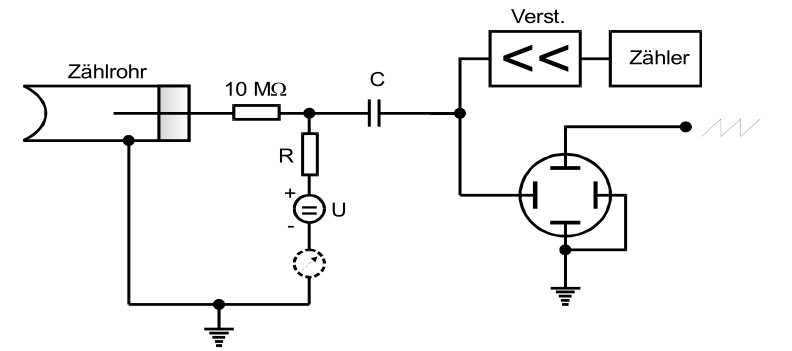
\includegraphics[width=0.8\textwidth]{images/skizze_4.png}
    \caption{Schaltkreis zur Messung der Kenndaten des Geiger-Müller Zählrohrs.\cite{V703}}
    \label{fig:schaltung}
\end{figure}

\subsection{Aufnahme der Charakteristik der Zählrohrs}
\label{ssec:charakteristik_durchführung}

Um den Plateauanstieg des Geiger-Müller Zählrohrs zu messen wird vor diesen eine Probe (hier $\prescript{204}{}{\text{Tl}}$) gestellt, welche $\beta$-Strahlung aussendet.
Nun wird in Abhängigkeit von der angelegten Spannung $U$ die Zählrate am Zähler abegelesen.
Dazu wird die Probe so plaziert, dass etwa 100 Impulse/s gemessen werden, da sonst die Totzeit mit beachtet werden muss.
Die Spannung sollte in einem passenden Bereich variiert werden, jedoch nicht ca. $\SI{700}{\volt}$ überschreiten, da höhere Spannungen das Zählrohr beschädigen können.
Die Messzeit pro Spannung sollte etwa $\SI{60}{\second}$ betragen, damit die Standardabweichung der Poisson-Verteilung bei unter $\SI{1}{\percent}$ bleibt.

Wird bei der Messung zusätzlich die Ionisierungsstromstärke gemessen, kann die freigesetzte Ladungsmenge pro einfallendem Teilchen bestimmt werden.

\subsection{Bestimmung der Totzeit}
\label{ssec:totzeit_durchführung}

Die Totzeit wird auf zwei verschiedene Arten bestimmt.

Für die Erste werden zwei Strahlungsquellen einzeln und zusammen gemessen.
Die Messzeit sollte in etwa doppelt so hoch wie zuvor sein, damit der statistische Fehler geringer ist.
Also wird als die Strahlung von Quelle 1 gemessen, dann wird Quelle 2 hinzugefügt ohne die erste Quelle zu bewegen.
Als letztes wird nur Quelle 2 vermessen.

Die zweite Messmethode verwendet nur eine Quelle und ein Oszilloskop.
Wenn die Strahlintensität der Quelle hoch genug ist, kann die Totzeit bestimmt werden indem die Zeitdifferenz zweier Impulse auf dem Oszilloskop abgelesen werden.